\subsubsection{\emph{Physical View}}
\label{subsubsec:physical-view}
\emph{Physical view} menggambarkan bagaimana sistem dipetakan ke infrastruktur fisik, seperti jaringan, server, dan perangkat keras. \emph{Physical view} memastikan bahwa sistem dapat beroperasi dengan baik dalam lingkungan yang telah ditentukan. \autoref{fig:deployment-diagram} menunjukkan \emph{deployment diagram} sistem pencatatan pengeluaran berbasis \emph{mobile} yang menggambarkan aplikasi \emph{mobile}, layanan \emph{backend}, API \emph{Gateway} (ngrok \emph{tunnel}), model internal, dan model \emph{deployed}. Pengguna akan berinteraksi langsung dengan aplikasi \emph{mobile} yang terpasang pada perangkat \emph{mobile}, yaitu TrackMyBills.apk. TrackMyBills.apk akan berkomunikasi dengan layanan \emph{backend} melalui API yang telah disediakan. Layanan \emph{backend} di-\emph{deploy} dalam Docker \emph{container} yang berjalan pada server yang telah disiapkan. Layanan \emph{backend} masih tidak dapat langsung diakses dari internet oleh TrackMyBills. Oleh karena itu, diperlukan \emph{tunnel} yang disediakan oleh ngrok untuk menghubungkan layanan \emph{backend} dengan TrackMyBills. Ngrok akan membuat \emph{tunnel} yang dapat diakses dari internet dan memberikan nama domain sehingga TrackMyBills dapat berkomunikasi dengan layanan \emph{backend}. Model internal merupakan bagian dari 
\begin{figure}[htbp]
    \centering
    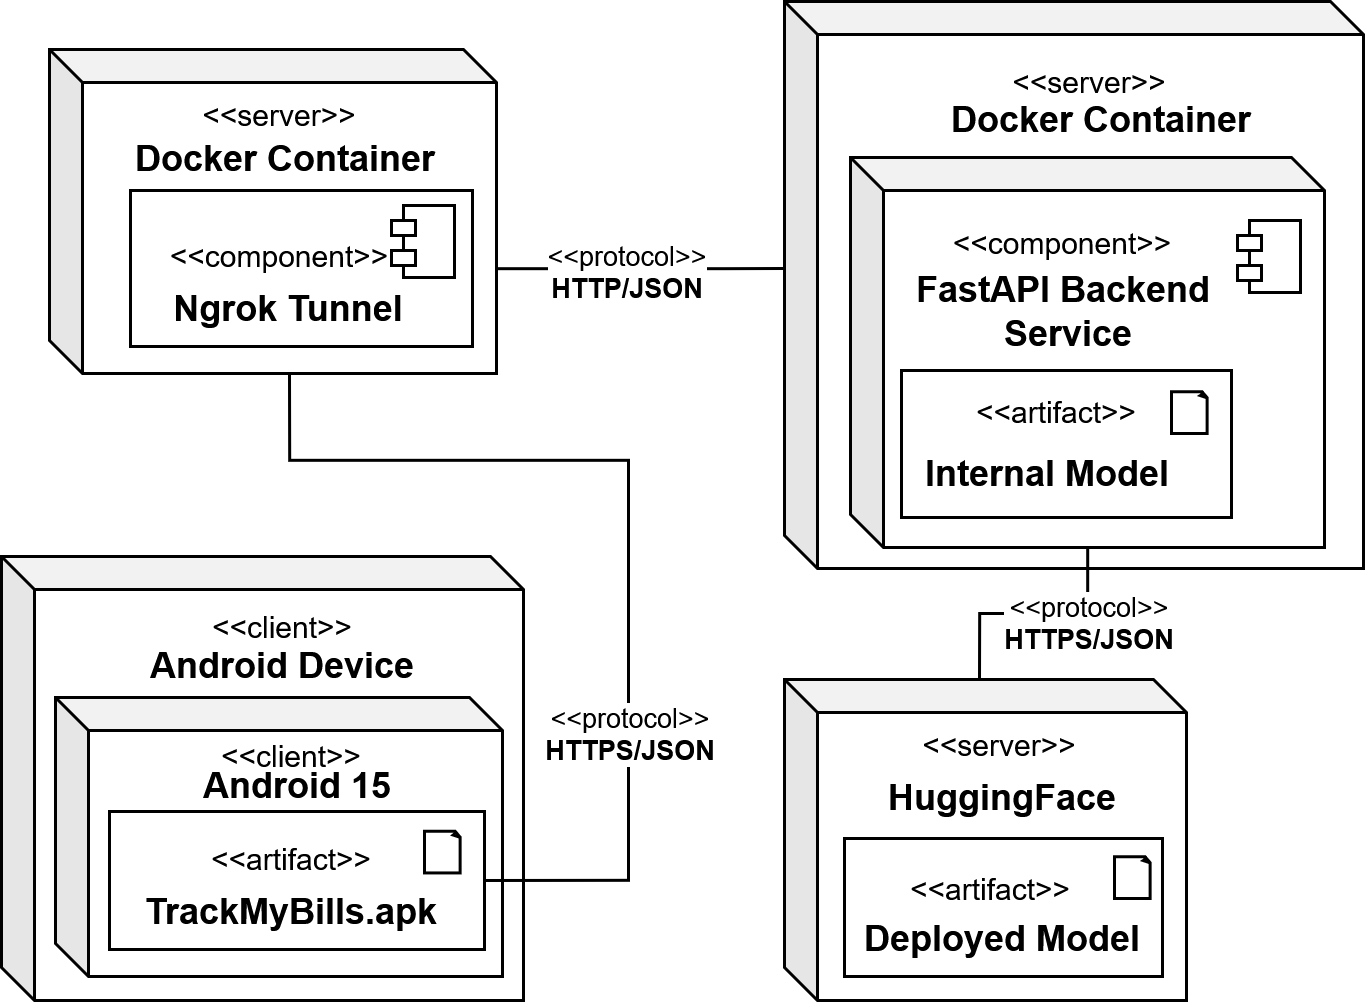
\includegraphics[width=1\textwidth]{images/deployment-diagram.png}
    \caption{\emph{Deployment diagram} sistem pencatatan pengeluaran berbasis \emph{mobile}}
    \label{fig:deployment-diagram}
\end{figure}